\part{Ayudantia 2}

\section{Parte 1}

Si tenemos un caso donde conocemos 2 puntos a alturas distinta:

\begin{figure}[H]
    \centering
    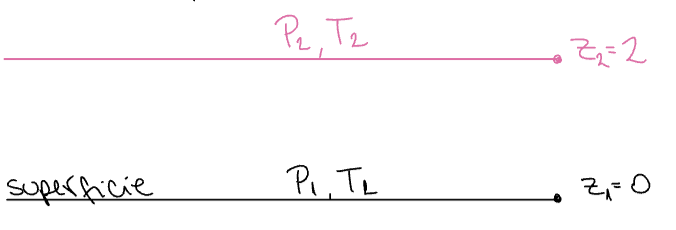
\includegraphics[width=0.5\textwidth]{imagenes/ayud_2_1.png}
    \label{fig:altura}
\end{figure}

Podemos determinar el agua precipitable se utiliza la siguiente formula:

\begin{equation}
    \Delta m_p = q_v \cdot p_a \cdot A \cdot \Delta Z
\end{equation}

$q_v$ se define como:

\begin{equation}
    q_v = 0.622 \cdot \frac{e}{p_a}
\end{equation}

Donde e es la presion de vapor y $p_a$ es la presion atmosferica.
\\ \\ 
Ademas, se tiene lo siguiente:

\begin{equation}
    HR = \frac{e}{e_s} \cdot 100
\end{equation}

Donde HR es la humedad relativa y $e_s$ es la presion de vapor de saturacion, de lo cual se obtiene:

\begin{equation}
    e_s = 611^(\frac{17.27 \cdot T}{237.3 + T})
\end{equation}

Los valores de e y $e_s$ son en pascales, donde las temperaturas son ingresadas en celcius.
\\ \\
Donde podemos calcular la presion del punto mas alto en variacion al punto base de referencia:

\begin{equation}
    P2 = P1 \cdot (\frac{T2}{T1})^(\frac{g}{\alpha \cdot Ra})
\end{equation}

Donde $\alpha$ ($\frac{C}{Km}$) es el gradiente de temperatura, Ra $\frac{J}{Kg \cdot K}$ es la constante de los gases y g es la gravedad.
\\ \\
Podemos conocer la temparatura en el punto de segun la temparatura en el punto 1:

\begin{equation}
    T2 = T1 + \alpha \cdot \Delta Z
\end{equation}

Ademas, es nesesario calcular la presion en el punto base de referencia segun la Ra y T:

\begin{equation}
    P1 = \frac{P1}{Ra \cdot T1}
\end{equation}

Lo mismo es nesesario hacer con P2.
\\ \\
Luego, como en este caso hay 2 puntos, hay que sacar el promedio de $q_v$ y Pa, obteniendo asi $\Delta m_p$.  

\section{parte 2}

Podemos obtener la vida util a partil de la seguridad:

\begin{equation}
    S = (1 - \frac{1}{T})^n
\end{equation}

Se define Gumbell como:

\begin{equation}
    X_T = \mu + K_t \cdot \sigma
\end{equation}

\begin{equation}
    K_t = \frac{y_t - y_n}{\sigma_n}
\end{equation}

\begin{equation}
    y_t = -\ln(\ln(\frac{T}{T-1}))
\end{equation}

Los valores n deben ser entregados.
\\ \\
La probabilidad de que la estructura falle mas de \textbf{X} veces es: